% Copyright (c) 2022 by Lars Spreng
% This work is licensed under the Creative Commons Attribution 4.0 International License. 
% To view a copy of this license, visit http://creativecommons.org/licenses/by/4.0/ or send a letter to Creative Commons, PO Box 1866, Mountain View, CA 94042, USA.

%~~~~~~~~~~~~~~~~~~~~~~~~~~~~~~~~~~~~~~~~~~~~~~~~~~~~~~~~~~~~~~~~~~~~~~~~~~~~~~
% You can add your packages and commands to the loadslides.tex file. 
% The files in the folder "styles" can be modified to change the layout and design of your slides.
% I have included examples on how to use the template below. 
% Some of it these examples are taken from the Metropolis template.
%~~~~~~~~~~~~~~~~~~~~~~~~~~~~~~~~~~~~~~~~~~~~~~~~~~~~~~~~~~~~~~~~~~~~~~~~~~~~~~

\documentclass[
11pt,notheorems,hyperref={pdfauthor=whatever}
]{beamer}


% Copyright (c) 2022 by Lars Spreng
% This work is licensed under the Creative Commons Attribution 4.0 International License. 
% To view a copy of this license, visit http://creativecommons.org/licenses/by/4.0/ or send a letter to Creative Commons, PO Box 1866, Mountain View, CA 94042, USA.

%~~~~~~~~~~~~~~~~~~~~~~~~~~~~~~~~~~~~~~~~~~~~~~~~~~~~~~~~~~~~~~~~~~~~~~~~~~~~~~
% Add your packages and commands to this file
%~~~~~~~~~~~~~~~~~~~~~~~~~~~~~~~~~~~~~~~~~~~~~~~~~~~~~~~~~~~~~~~~~~~~~~~~~~~~~~

%~~~~~~~~~~~~~~~~~~~~~~~~~~~~~~~~~~~~~~~~~~~~~~~~~~~~~~~~~~~~~~~~~~~~~~~~~~~~~~
\RequirePackage{palatino}
\RequirePackage[utf8]{inputenc}
\RequirePackage[T1]{fontenc}

\usefonttheme{serif}

\usepackage{styles/elegantmacros}
\usefolder{styles}
\usetheme[style=blue]{elegant}

\newcommand{\makepart}[1]{ % For convenience
\part{#1} \frame{\partpage}
} 

%~~~~~~~~~~~~~~~~~~~~~~~~~~~~~~~~~~~~~~~~~~~~~~~~~~~~~~~~~~~~~~~~~~~~~~~~~~~~~~

%~~~~~~~~~~~~~~~~~~~~~~~~~~~~~~~~~~~~~~~~~~~~~~~~~~~~~~~~~~~~~~~~~~~~~~~~~~~~~~
% Figures
\RequirePackage{booktabs}
\RequirePackage{colortbl}
\RequirePackage{ragged2e}
\RequirePackage{schemabloc}
%\RequirePackage{natbib}
\RequirePackage{caption}
\RequirePackage{subcaption}
\RequirePackage{tabularx}
\RequirePackage{array}
\RequirePackage{multirow}
\usepackage[
  style=authoryear, 
]{biblatex}
\RequirePackage{xcolor}
\addbibresource{references.bib}
\newcolumntype{Y}{>{\centering\arraybackslash}X}

%~~~~~~~~~~~~~~~~~~~~~~~~~~~~~~~~~~~~~~~~~~~~~~~~~~~~~~~~~~~~~~~~~~~~~~~~~~~~~~

%~~~~~~~~~~~~~~~~~~~~~~~~~~~~~~~~~~~~~~~~~~~~~~~~~~~~~~~~~~~~~~~~~~~~~~~~~~~~~~
% Figures
\RequirePackage{wrapfig}
\RequirePackage{pgfplots}
\RequirePackage{graphicx}
\RequirePackage{adjustbox}
\RequirePackage{environ}
\pgfplotsset{compat=1.18  }

\makeatletter
\newsavebox{\measure@tikzpicture}
\NewEnviron{scaletikzpicturetowidth}[1]{%
  \def\tikz@width{#1}%
  \def\tikzscale{1}\begin{lrbox}{\measure@tikzpicture}%
  \BODY
  \end{lrbox}%
  \pgfmathparse{#1/\wd\measure@tikzpicture}%
  \edef\tikzscale{\pgfmathresult}%
  \BODY
}
\makeatother
%~~~~~~~~~~~~~~~~~~~~~~~~~~~~~~~~~~~~~~~~~~~~~~~~~~~~~~~~~~~~~~~~~~~~~~~~~~~~~~

%~~~~~~~~~~~~~~~~~~~~~~~~~~~~~~~~~~~~~~~~~~~~~~~~~~~~~~~~~~~~~~~~~~~~~~~~~~~~~~
% Maths 
\RequirePackage{textcomp}
\RequirePackage{amsmath} 
\RequirePackage{amsthm}
\RequirePackage{mathtools}
\RequirePackage{braket}
%\RequirePackage{bbm}
%\RequirePackage{algorithm}
%\RequirePackage[osf,sc]{mathpazo}
%\RequirePackage{pifont}
%\newcommand{\xmark}{\ding{55}}%
%\numberwithin{equation}{section}
\DeclareMathOperator*{\argmax}{arg\,max}
\DeclareMathOperator*{\argmin}{arg\,min}

\setbeamertemplate{theorems}[numbered] % to number

\theoremstyle{definition}
\newtheorem{fact}{Fact}[section]
\newtheorem{examp}{Example}[section]

\theoremstyle{plain}
\newtheorem{definition}{Definition}[section]
\newtheorem{proposition}{Proposition}
\newtheorem{theorem}{Theorem}
\newtheorem{assumption}{Assumption}

\providecommand{\H}{\mathscr{H}}      
\providecommand{\E}{\mathbb{E}}
\makeatletter
\def\munderbar#1{\underline{\sbox\tw@{$#1$}\dp\tw@\z@\box\tw@}}
\makeatother

%~~~~~~~~~~~~~~~~~~~~~~~~~~~~~~~~~~~~~~~~~~~~~~~~~~~~~~~~~~~~~~~~~~~~~~~~~~~~~~
%Commands
\newcommand{\importanttext}[1]{\Large #1 \normalsize}
\newcommand{\crt}[1]{a_{#1}^{\dagger}}
\newcommand{\ani}[1]{a_{#1}}
\newcommand{\vac}{\ket{0}}
\newcommand{\gs}{\ket{\Phi_0}}
\newcommand{\exed}[2]{\ket{\Phi_{#1}^{#2}}}

\newcommand{\inner}[3]{\bra{#1}#2\ket{#3}}
\newcommand{\innerAS}[3]{\inner{#1}{#2}{#3}_{\text{AS}}}
\newcommand{\mathset}[1]{\{ #1 \}}
\newcommand{\ord}[2]{#1^{(#2)}}
\newcommand{\energyref}{E_0^{\text{ref}}}
\newcommand{\psum}{\sideset{}{'}\sum}

\newcommand{\spinop}[1]{\hat{S}_{#1}}
\newcommand{\pplus}[1]{\hat{P}_{#1}^{+}}
\newcommand{\pminus}[1]{\hat{P}_{#1}^{-}}
\newcommand{\numberop}[1]{\hat{N}_{#1}}
\newcommand{\hatreefock}[1]{#1^{\text{HF}}}
\newcommand{\comment}[1]{\textcolor{red}{#1}}
\newcommand{\functional}[1]{\[ #1 \}}

% Colors
\definecolor{Green}{RGB}{20, 128, 10}
\definecolor{Red}{RGB}{153, 22, 8} % Loads packages and some defined commands

\title[
% Text entered here will appear in the bottom middle
]{FYS4480 Oral exam, midterm one and two}

\subtitle{Helium and Beryllium using CIS and Hartree-Fock, pairing model}

\author[
% Text entered here will appear in the bottom left corner
]{
    Håkon Kvernmoen
}

\institute{
    University of Oslo}
\date{\today}

\begin{document}

% Generate title page
{
\setbeamertemplate{footline}{} 
\begin{frame}
  \titlepage
\end{frame}
}
\addtocounter{framenumber}{-1}

% You can declare different parts as a parentof sections
% \begin{frame}{Part I: Demo Presentation Part}
%     \tableofcontents[part=1]
% \end{frame}
% \begin{frame}{Part II: Demo Presentation Part 2}
%     \tableofcontents[part=2]
% \end{frame}

% \makepart{Demo Part}

% \section{Introduction}
% \begin{frame}
% \begin{itemize}
%     \item This template provides an elegant and minimalistic layout for beamer slides. Hence the name \alert{\textbf{Elegant Slides}}.
%     \item I created Elegant Slides because I wasn't satisfied with any of the existing Beamer templates, which look slightly different than Elegant Slides.
%     \item My goal was to create a layout that is \alert{\textbf{simplistic but beautiful}} and focuses on the content, rather than crowding each slide with lots of different coloured boxes.
%     \item I designed Elegant Slides for \alert{\textbf{lecture notes and technical presentations}} but it can be used for any kind of talk. 
% \end{itemize}
     
% \end{frame}

\begin{frame}
    \frametitle{Setup}
    Represent states using creation $\crt{p}$ and annihilation $\ani{q}$ operators (occupation representation/second quantization), obeying
    \begin{align*}
        \mathset{\crt{p},\ani{q}} = \delta_{pq},\hspace{20px}\mathset{\crt{p},\crt{q}} = \mathset{\ani{p},\ani{q}} = 0
    \end{align*}
    $p$ and $q$ are sets of relevant quantum numbers. We need to pick a single particle (SP) computational basis, having $n$ possible single particle states.
    \begin{align*}
        \text{3D HO:}\hspace{20px}p = \mathset{n_r,l,m_l,s,m_s},\hspace{20px} \crt{p} \vac = \ket{p} \longrightarrow \psi_p(\bold{x}) = \psi_{n_r l m}(r, \theta, \phi) = \ldots 
    \end{align*} 
    Need a Hamiltonian to solve $\hat{H} = \hat{H}_0 + \hat{V}$, with $\hat{H}_0$ representing single particle energy contributions, and $\hat{V}$ interactions.
    \\[10pt]
    Often start with an $N$-particle ground state ansatz $\ket{\Phi_0} = \crt{1},\ldots \crt{N} \vac$.
    \\[10pt]
    And consider excitations of this
    \begin{align*}
        \text{1p1h}\hspace{20px}&\exed{i}{a} = \crt{a}\ani{i}\gs \\
        \text{2p2h}\hspace{20px}&\exed{ij}{ab} = \crt{a}\crt{b}\ani{j}\ani{i}\gs  \\
        \text{NpNh}\hspace{20px}&\exed{ij\ldots}{ab\ldots} = \crt{a}\crt{b}\ldots\ani{j}\ani{i}\gs 
    \end{align*}
\end{frame}


\subsection{FCI}
\begin{frame}
    \frametitle{Full configuration interaction (FCI)}

    Start with $N$ particle ground state ansatz $\ket{\Phi_0}$.
    \\[10pt]
    Not an eigenstate of $\hat{V}$ and therefor not the true ground state of the system.
    \\[10pt]
    By considering every possible $N$ particle state in our system (using $\mathset{\crt{1},\ldots,\crt{N},\ldots,\crt{n}}$), we can construct our ground state $\ket{\Psi_0}$ as a linear combination of excited states.
    \begin{align*}
        \ket{\Psi_0} = C_0 + \sum_{ai} C_i^a \exed{i}{a} + \sum_{ai} C_{ij}^{ab} \exed{ij}{ab} + \ldots
    \end{align*} 
    \\[10pt] 
    Normally solved by considering the Hamiltonian in matrix representation, with elements $H_{XY} = \inner{\Phi_X}{\hat{H}}{\Phi_Y}$, with $X, Y \in \mathset{\text{0p0h},\text{1p1h}\ldots\text{NpNh}}$, giving the eigenvalue problem 
    \begin{align*}
        H \bold{c} = E\bold{c}
    \end{align*}
    When solved, the smallest eigenvalue $\ord{E}{0}$ will yield the ground state energy, and $\ket{\Psi_0}$ can be found by considering the eigenvectors $\ord{\bold{c}}{0} = (C_0, C_{i}^{a} \ldots C_{ij}^{ab} \ldots \ldots C_{ij\ldots}^{ab\ldots})$. Excited states can also be found by considering the other eigenvalues and vectors $\ord{E}{i}, \ord{\bold{c}}{i}$.
\end{frame}

\subsection{FCI}
\begin{frame}
    Example, pairing interaction: $\hat{V}$ only works between spin-paired states at the same energy level. We let $p = 1, 2, 3, 4$ denote energy levels, with SP states also having a spin $\sigma = \pm$, a total of $n = 8$ SP states. 
    \begin{align*}
        \hat{H} = \hat{H}_0 + \hat{V},\hspace{20px} \hat{H}_0 = \sum_{p\sigma} (p-1)\crt{p\sigma}\ani{p\sigma}, \hspace{20px}\hat{V} = -\frac{1}{2}g\sum_{pq}\crt{p+}\crt{p-}\ani{q-}\ani{q+}
    \end{align*}
    Diagonal SP Hamiltonian $\hat{H}_0$ and two body interaction $\hat{V}$. Consider $N = 4$ particles with total spin $S = 0$, writing $\ket{PQ} = \ket{p+p-q+q-}$ we have a total of six different many body states.
    \begin{align*}
        \text{0p0h}&\hspace{20px} \ket{12}  \\
        \text{2p2h}&\hspace{20px} \ket{13}, \ket{14}, \ket{23}, \ket{24} \\  
        \text{4p4h}&\hspace{20px} \ket{34}
    \end{align*}
    By setting up the matrix $\inner{KL}{\hat{H}}{RS}$, we get a small eigenvalue problem of a $6 \times 6$ matrix.
\end{frame}

\subsection{FCI}
\begin{frame}
    \begin{figure}
        \centering
        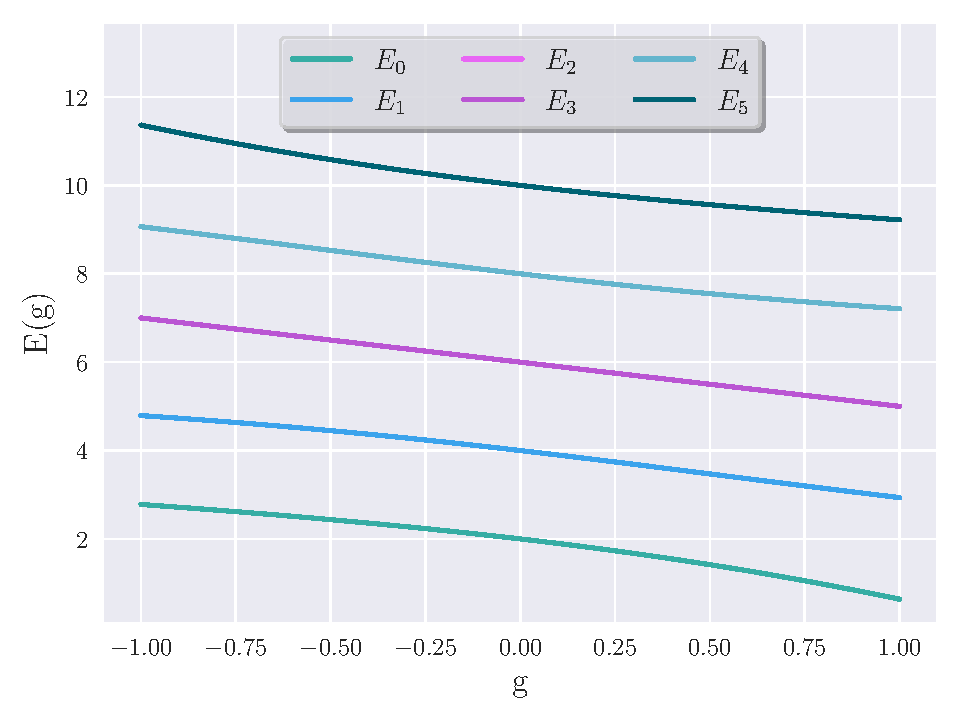
\includegraphics[width=0.75\linewidth]{figs/FCI.pdf}
    \end{figure}
    But there is a problem...
\end{frame}

\subsection{FCI}
\begin{frame}
    For all but very simple problems, this approach is unfeasible. In general, we have to consider 
    \begin{align*}
        \binom{n}{N} = \frac{n!}{N!(n-N)!}
    \end{align*}
    many body states. Taking our pairing model example, lifting the $S = 0$ restriction yields 70 different states. This is still possible, but increasing both $n$ and $N$ results in disaster
    
    \begin{table}
        \begin{tabular}{c|l|l|l|l}
        $N \downarrow /n \rightarrow$ & 8    & 32       & 64        & 128       \\
        \hline
        4     & $70$ & $10^{4}$ & $10^{5}$  & $10^{7}$  \\
        8     &      & $10^{7}$ & $10^{9}$  & $10^{12}$ \\
        16    &      & $10^{8}$ & $10^{14}$ & $10^{19}$ \\
        32    &      &          & $10^{18}$ & $10^{30}$
        \end{tabular}
        \caption{NB: Order of magnitude values}
    \end{table}
\end{frame}

\subsection{FCI}
\begin{frame}
    \textcolor{Green}{\importanttext{Pros:}}
    \begin{itemize}
        \item Provides exact solutions within a truncated basis set
        \item Understandable and relatively easy to set up 
        \item Excited states thrown into the bargain
    \end{itemize}
    \vspace{20px}
    \textcolor{Red}{\importanttext{Cons:}}
    \begin{itemize}
        \item Computational complexity, bad scaling
        \item Only possible for tiny systems, with few states and particles.
        \item Practically only a benchmarking tool
    \end{itemize}
\end{frame}

\begin{frame}
    \frametitle{Configuration Interaction (CI)}
    Follows the same methodology as FCI, but due to its large computational time, the many body states are also truncated.
    \\[10pt]
    Different truncation levels can be chosen, for instance only include (in addition to $\gs$) 1p1h excitations (CIS) or 2p2h excitations (CID).
    \\[10pt]
    Truncation relies on an a priori ranking of the importance of different excited states, which contributions to include might not be obvious.
    \\[10pt]
    Considering our paring model example, we can exclude the 4p4h ($\ket{34}$) contributions from $\inner{KL}{\hat{H}}{RS}$, giving only the ground state ansatz and 2p2h excitations.
    \\[10pt]
    This reduces the matrix $6 \times 6 \xrightarrow{} 5 \times 5$, showing how truncation is beneficial from a computational point of view.
\end{frame}

\subsection{CI}
\begin{frame}
    \begin{figure}
        \begin{subfigure}{.49\textwidth}
            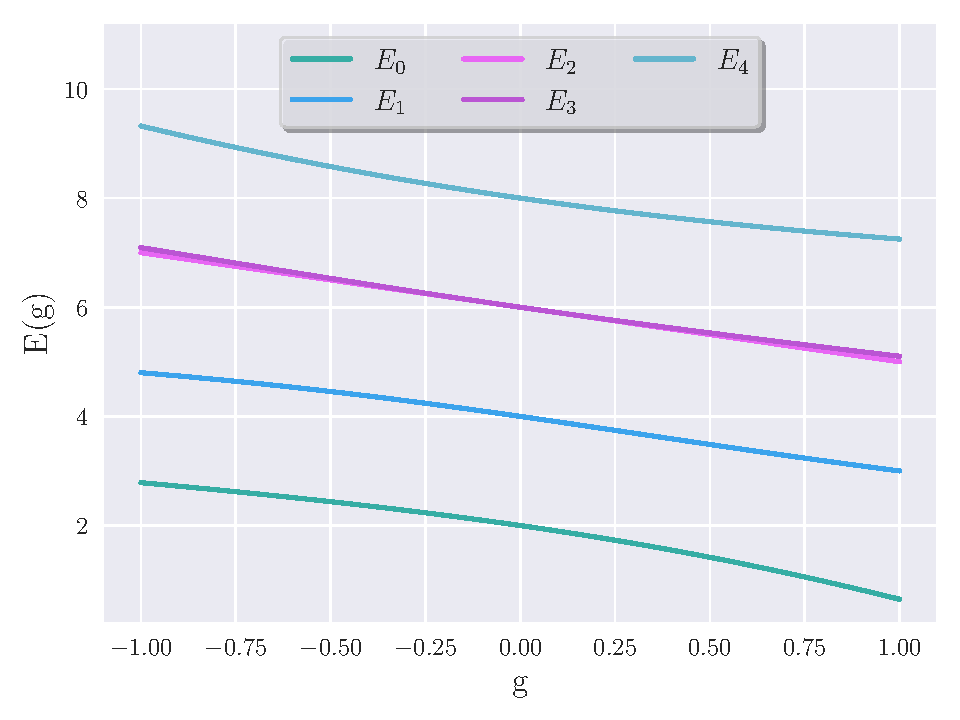
\includegraphics[width=\linewidth]{figs/CID.pdf}
        \end{subfigure}
        \hfill
        \begin{subfigure}{.49\textwidth}
            \centering
            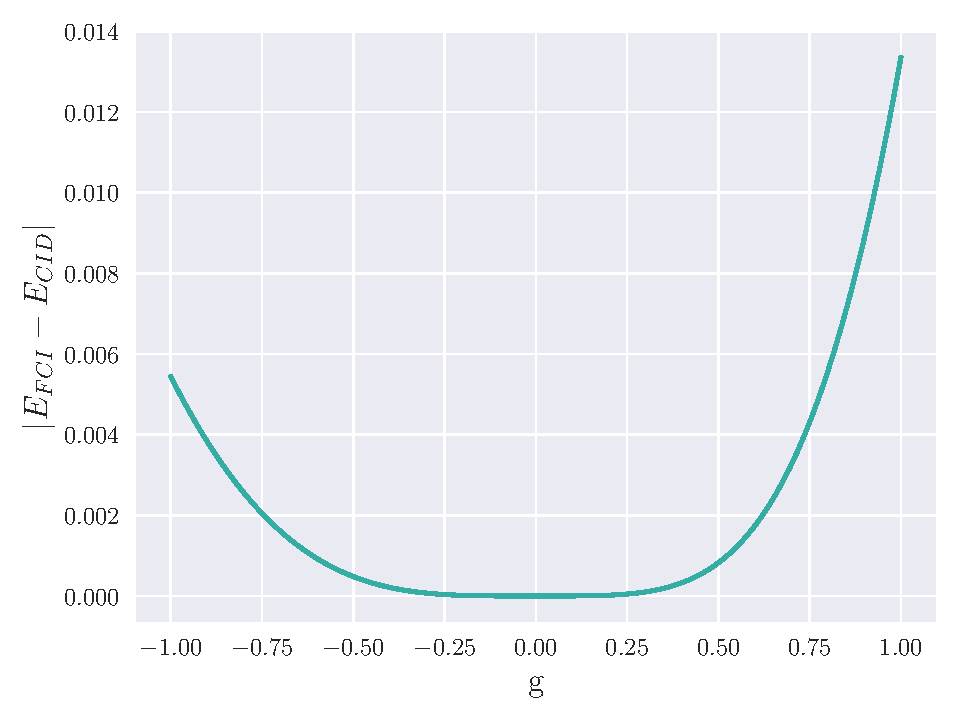
\includegraphics[width=\linewidth]{figs/FCI_CID_diff.pdf}
        \end{subfigure}
    \end{figure}
\end{frame}


\subsection{CI}
\begin{frame}
    \textcolor{Green}{\importanttext{Pros:}}
    \begin{itemize}
        \item Understandable and relatively easy to set up 
        \item Excited states thrown into the bargain
        \item Reduces the problem of FCI
        \item When adding contributions, the exact energy is approached.
    \end{itemize}
    \vspace{20px}
    \textcolor{Red}{\importanttext{Cons:}}
    \begin{itemize}
        \item Still quite computationally expensive
        \item Bad scaling for higher contributions
        \item What contributions to include might not be obvious
    \end{itemize}
\end{frame}

\begin{frame}
    \frametitle{Hartree-Fock (HF)}
    Hartree-Fock methods approximate two body interactions as a mean field potential.
    
    \begin{align*}
        \inner{\Phi_0}{\hat{H}}{\Phi_0} \equiv 
    \end{align*}
\end{frame}

\begin{frame}{Custom Title}{Custom Subsection with Footnote}
    This frame has a custom title and a custom subtitle.\footnote{This is a footnote. See also \textcite{example_2022}. }
\end{frame}

\subsection{Typographics}
\begin{frame}
    These examples follow the Metropolis Theme
    \begin{itemize}
        \item Regular
        \item \alert{Alert}
        \item \textit{Italic}
        \item \textbf{Bold}
    \end{itemize}
\end{frame}

\subsection{Lists}

\begin{frame}
    \begin{columns}[T,onlytextwidth]
    \column{0.33\textwidth}
      \textbf{Items}
      \begin{itemize}
        \item Cats 
        \begin{itemize}
            \item British Shorthair
        \end{itemize}
        \item Dogs \item Birds
      \end{itemize}

    \column{0.33\textwidth}
      \textbf{Enumerations}
      \begin{enumerate}
        \item First 
        \begin{enumerate}
            \item First subpoint
        \end{enumerate}
        \item Second \item Last
      \end{enumerate}

    \column{0.33\textwidth}
      \textbf{Descriptions}
      \begin{description}
        \item[Apples] Yes \item[Oranges] No \item[Grappes] No
      \end{description}
\end{columns}
\end{frame}

\subsection{Table}
\begin{frame}
    \begin{table}
        \caption{Largest cities in the world (source: Wikipedia)}
        \begin{tabular}{@{} lr @{}}
          \toprule
          City & Population\\
          \midrule
          Mexico City & 20,116,842\\
          Shanghai & 19,210,000\\
          Peking & 15,796,450\\
          Istanbul & 14,160,467\\
          \bottomrule
        \end{tabular}
        \hspace*{1cm}
            \setlength\extrarowheight{3pt}
        \begin{tabular}{|lr|}
          \hline
          \rowcolor{primary}\color{white}City & \color{white}Population\\
          \hline
          Mexico City & 20,116,842\\
          Shanghai & 19,210,000\\
          Peking & 15,796,450\\
          Istanbul & 14,160,467\\
          \hline
        \end{tabular}
    \end{table}
\end{frame}

\subsection{Figures}
\begin{frame}
    \begin{figure}[htbp]
        \centering
        \caption{Plot of $y=x^2$}
        \begin{tikzpicture}
            \begin{axis}[
            legend columns=3,
            legend style={at={(0.5,-0.3)},anchor=north},
            width = \textwidth,
            height = 2.5in,
            xmin = -3, 
            xmax = 3,
            ymin = 0,
            ymax = 10,
            ]
                \addplot[primary] {x^2};
                        \addlegendentry{$x^2$}
            \end{axis}
        \end{tikzpicture}
    \end{figure}

\end{frame}

\subsection{Blocks}
\begin{frame}

   \centering
	\begin{minipage}[b]{0.5\textwidth}

	  \begin{block}{Default}
        Block content.
      \end{block}

      \begin{alertblock}{Alert}
        Block content.
      \end{alertblock}

      \begin{exampleblock}{Example}
        Block content.
      \end{exampleblock}      
      
	\end{minipage}	
\end{frame}

\section{Maths}
\subsection{Equations}
\begin{frame}
    \begin{itemize}
        \item A numbered equation:
        \begin{equation}
            y_t = \beta x_t + \varepsilon_t
        \end{equation}
         \item Another equation:
        \begin{equation*}
            \mathbf{Y} = \boldsymbol{\beta} \mathbf{X} + \boldsymbol{\varepsilon}_t
        \end{equation*}
    \end{itemize}
\end{frame}

\subsection{Theorem}
\begin{frame}
    \begin{itemize}
        \item Theorems are numbered consecutively.
    \end{itemize}
    \begin{theorem}[Example Theorem]
         Given a discrete random variable X, which takes values in the alphabet $\mathcal{X}$ and is distributed according to  $p:{\mathcal {X}}\to [0,1]$:
            \begin{equation}
                \mathrm {H} (X):=-\sum _{x\in {\mathcal {X}}}p(x)\log p(x)=\mathbb {E} [-\log p(X)]
            \end{equation}
    \end{theorem}
\end{frame}

\begin{frame}{}{Definitions}
    \begin{itemize}
        \item Definition numbers are prefixed by the section number in the respective part.
    \end{itemize}
     \begin{definition}[Example Definition]
         Given a discrete random variable X, which takes values in the alphabet $\mathcal{X}$ and is distributed according to  $p:{\mathcal {X}}\to [0,1]$:
            \begin{equation}
                \mathrm {H} (X):=-\sum _{x\in {\mathcal {X}}}p(x)\log p(x)=\mathbb {E} [-\log p(X)]
            \end{equation}
    \end{definition}
\end{frame}

\begin{frame}{}{Examples}
    \begin{itemize}
        \item Examples are numbered as definitions.
    \end{itemize}
    \begin{examp}[Example Theorem]
         Given a discrete random variable X, which takes values in the alphabet $\mathcal{X}$ and is distributed according to  $p:{\mathcal {X}}\to [0,1]$:
            \begin{equation}
                \mathrm {H} (X):=-\sum _{x\in {\mathcal {X}}}p(x)\log p(x)=\mathbb {E} [-\log p(X)]
            \end{equation}
    \end{examp}
\end{frame}

\makepart{Demo Presentation Part 2}

\section{Section}
\subsection{Subsection}
\subsubsection{Subsubsection}
\subsubsection{Subsubsection}
\subsection{Subsection}
\subsubsection{Subsubsection}
\subsubsection{Subsubsection}
\section{Section}
\subsection{Subsection}
\subsubsection{Subsubsection}
\subsubsection{Subsubsection}
\subsection{Subsection}
\subsubsection{Subsubsection}
\subsubsection{Subsubsection}

\begin{frame}[allowframebreaks]{References}
    \printbibliography
\end{frame}
\end{document}